\documentclass[12pt,a4paper]{article}
\usepackage{float}
\usepackage{amsfonts}
\usepackage{amsmath}
\usepackage{amssymb}
\usepackage{amsthm}
\usepackage{caption}
\usepackage{fontenc}
\usepackage{graphicx}
\usepackage{ucs}
\usepackage[utf8]{inputenc}
\usepackage[left=1.00cm, right=1.00cm, top=1.00cm, bottom=2.00cm]{geometry}
\usepackage{makeidx}
\usepackage{multicol}
\usepackage{pst-all}
\usepackage{rotating}
\usepackage{subfigure}
\usepackage{upgreek}
\usepackage[USenglish]{babel}
\usepackage[ref,nobreak]{cite}
\usepackage{xcolor}
\usepackage{cancel}
\usepackage{listings}
\usepackage[colorlinks=true,pagebackref=true,breaklinks=true]{hyperref}


\newcommand {\hsm}          {\ensuremath{H_{\text{SM}}}}
\newcommand {\chh}          {\ensuremath{H^{\pm}}}
\newcommand {\ttbar}        {\ensuremath{t \bar{t}}}
\newcommand {\ttbarbbbar}   {\ensuremath{t \bar{t} b \bar{b}}}
\newcommand {\signalgbth}   {\ensuremath{g b \rightarrow t \chh}}
\newcommand {\signalggtbh}  {\ensuremath{g g \rightarrow t b \chh}}
\newcommand {\nmssmtools}   {\tt NMSSMTools-5.0.0}

\newcommand {\pythia}       {{\tt PYTHIA8-8.2.26} \cite{Sjostrand:2006za}}
\newcommand {\pyth}         {\tt PYTHIA8}

\newcommand {\madgraph}     {\tt MadGraph\_aMC@NLO-2.5.5 \cite{Alwall:2014hca}}
\newcommand {\mg}           {\tt MadGraph5}

\newcommand {\fastjet}      {{\tt fastjet-3.3.0} \cite{Cacciari2012}}
\newcommand {\fj}           {\tt fastjet}

\newcommand {\cernroot}     {{\tt root-6.08.06} \cite{BRUN199781}}

\newcommand {\heptoptagger} {{\tt HEPTopTagger2} \cite{Plehn:2011tg,Kasieczka:2015jma,Plehn:2010st,Plehn:2009rk}}
\newcommand {\toptag}       {\tt HEPTopTagger}

\newcommand {\cajet}        {{\tt Cambridge/Aachen} (C/A) \cite{Dokshitzer:1997in}}
\newcommand {\akjet}        {Anti-$k_t$ \cite{1126-6708-2008-04-063}}

\definecolor{mGreen}{rgb}{0,0.6,0}
\definecolor{mGray}{rgb}{0.5,0.5,0.5}
\definecolor{mPurple}{rgb}{0.58,0,0.82}
\definecolor{backgroundColour}{rgb}{0.95,0.95,0.92}

\definecolor{mred}{rgb}{0.5,0.0,0.0}
\definecolor{mgreen}{rgb}{0.0,0.5,0.0}
\definecolor{mblue}{rgb}{0.0,0.0,0.5}
\definecolor{myellow}{rgb}{0.5,0.5,0.0}
\definecolor{mpink}{rgb}{0.5,0.0,0.5}
\definecolor{mcyan}{rgb}{0.0,0.5,0.5}
\definecolor{mblack}{rgb}{0.0,0.0,0.0}

\lstdefinestyle{CStyle}{
%	backgroundcolor=\color{backgroundColour},
	commentstyle=\color{mGreen},
	keywordstyle=\color{magenta},
	numberstyle=\tiny\color{mGray},
	stringstyle=\color{mPurple},
	basicstyle=\footnotesize,
	breakatwhitespace=false,
	breaklines=true,
	captionpos=b,
	keepspaces=true,
	numbers=left,
	numbersep=5pt,
	showspaces=false,
	showstringspaces=false,
	showtabs=false,
	tabsize=2,
	language=C
}

\begin{document}
	akgdkjahgsd

$e^{i \pi}=1$

    The ratio $\frac{m_0}{E_0}$ determines the length scale to resolve the jet,
    a condition $m_{0}<E_{0}$ is very important for the consistency of our method.\\
    When the ratio is too large, the prongs are smeared towards the edges like in \autoref{fig:case9}.\\
    When the ratio is too small, the prongs are not well resolved like in \autoref{fig:case1}.\\
    A ratio of $\frac{m_0}{E_0}=\frac{1}{2}$ [\autoref{fig:case5}] was chosen as it ``seems'' to correctly resolve the jet, probably this ratio can also be optimized.
    
    \begin{figure}
        \begin{center}
            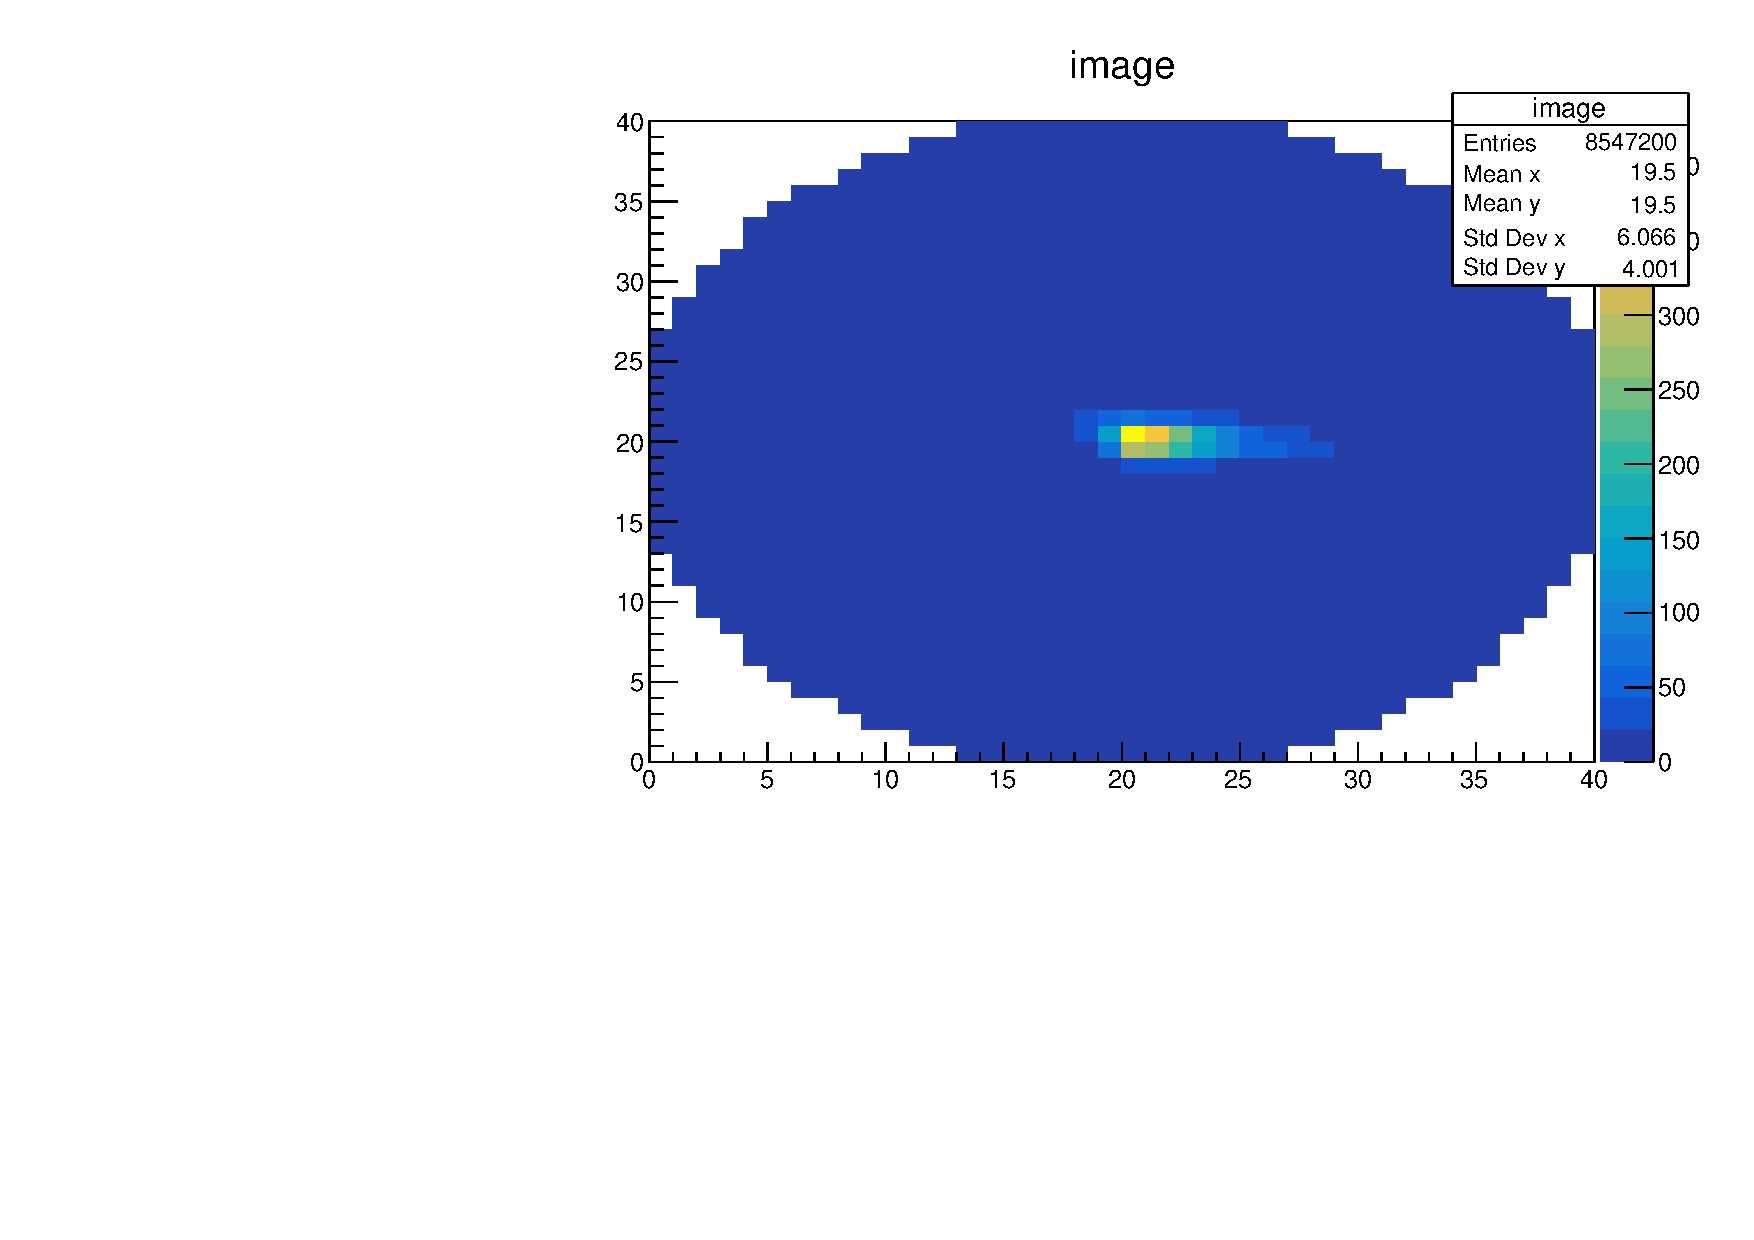
\includegraphics[width=0.32\textwidth]{./NoNorm/imageQCD.pdf}
            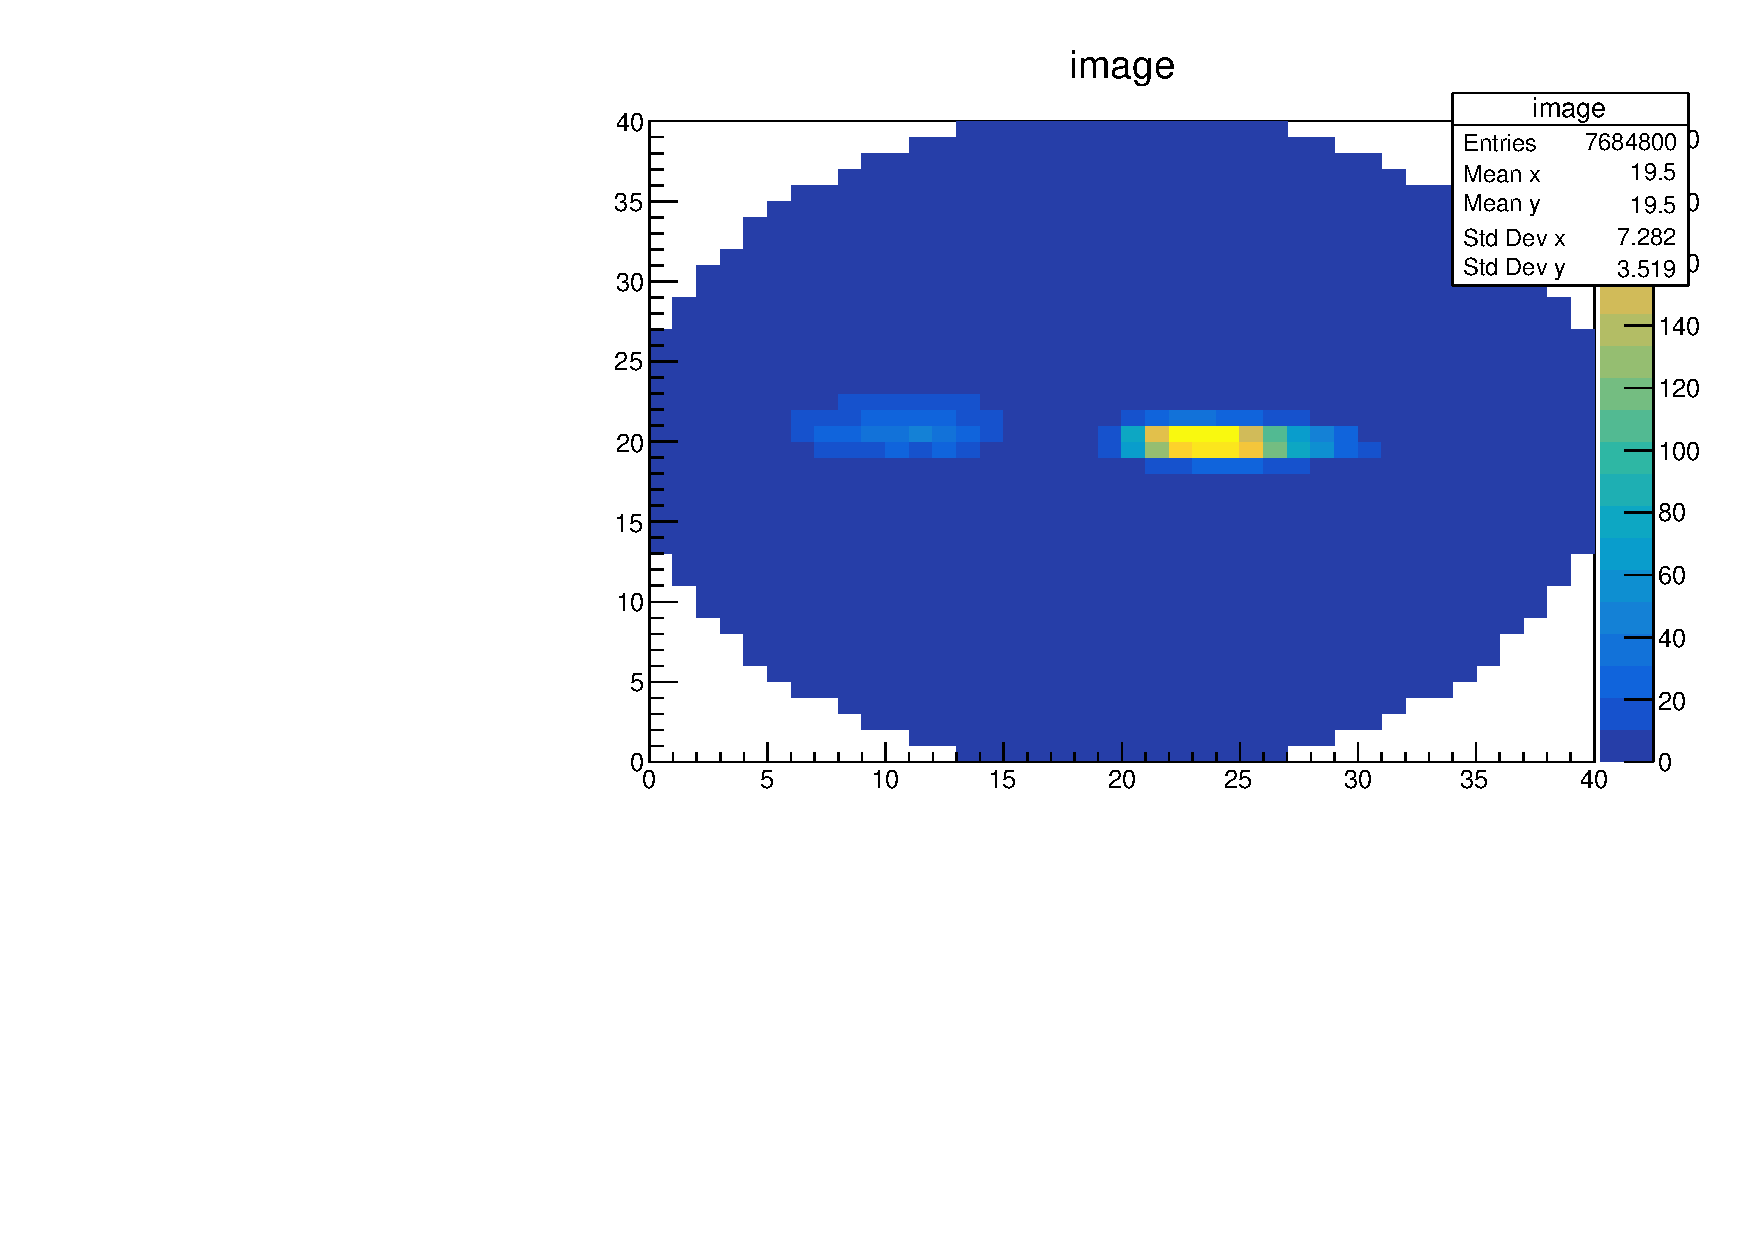
\includegraphics[width=0.32\textwidth]{./NoNorm/imageW.pdf}
            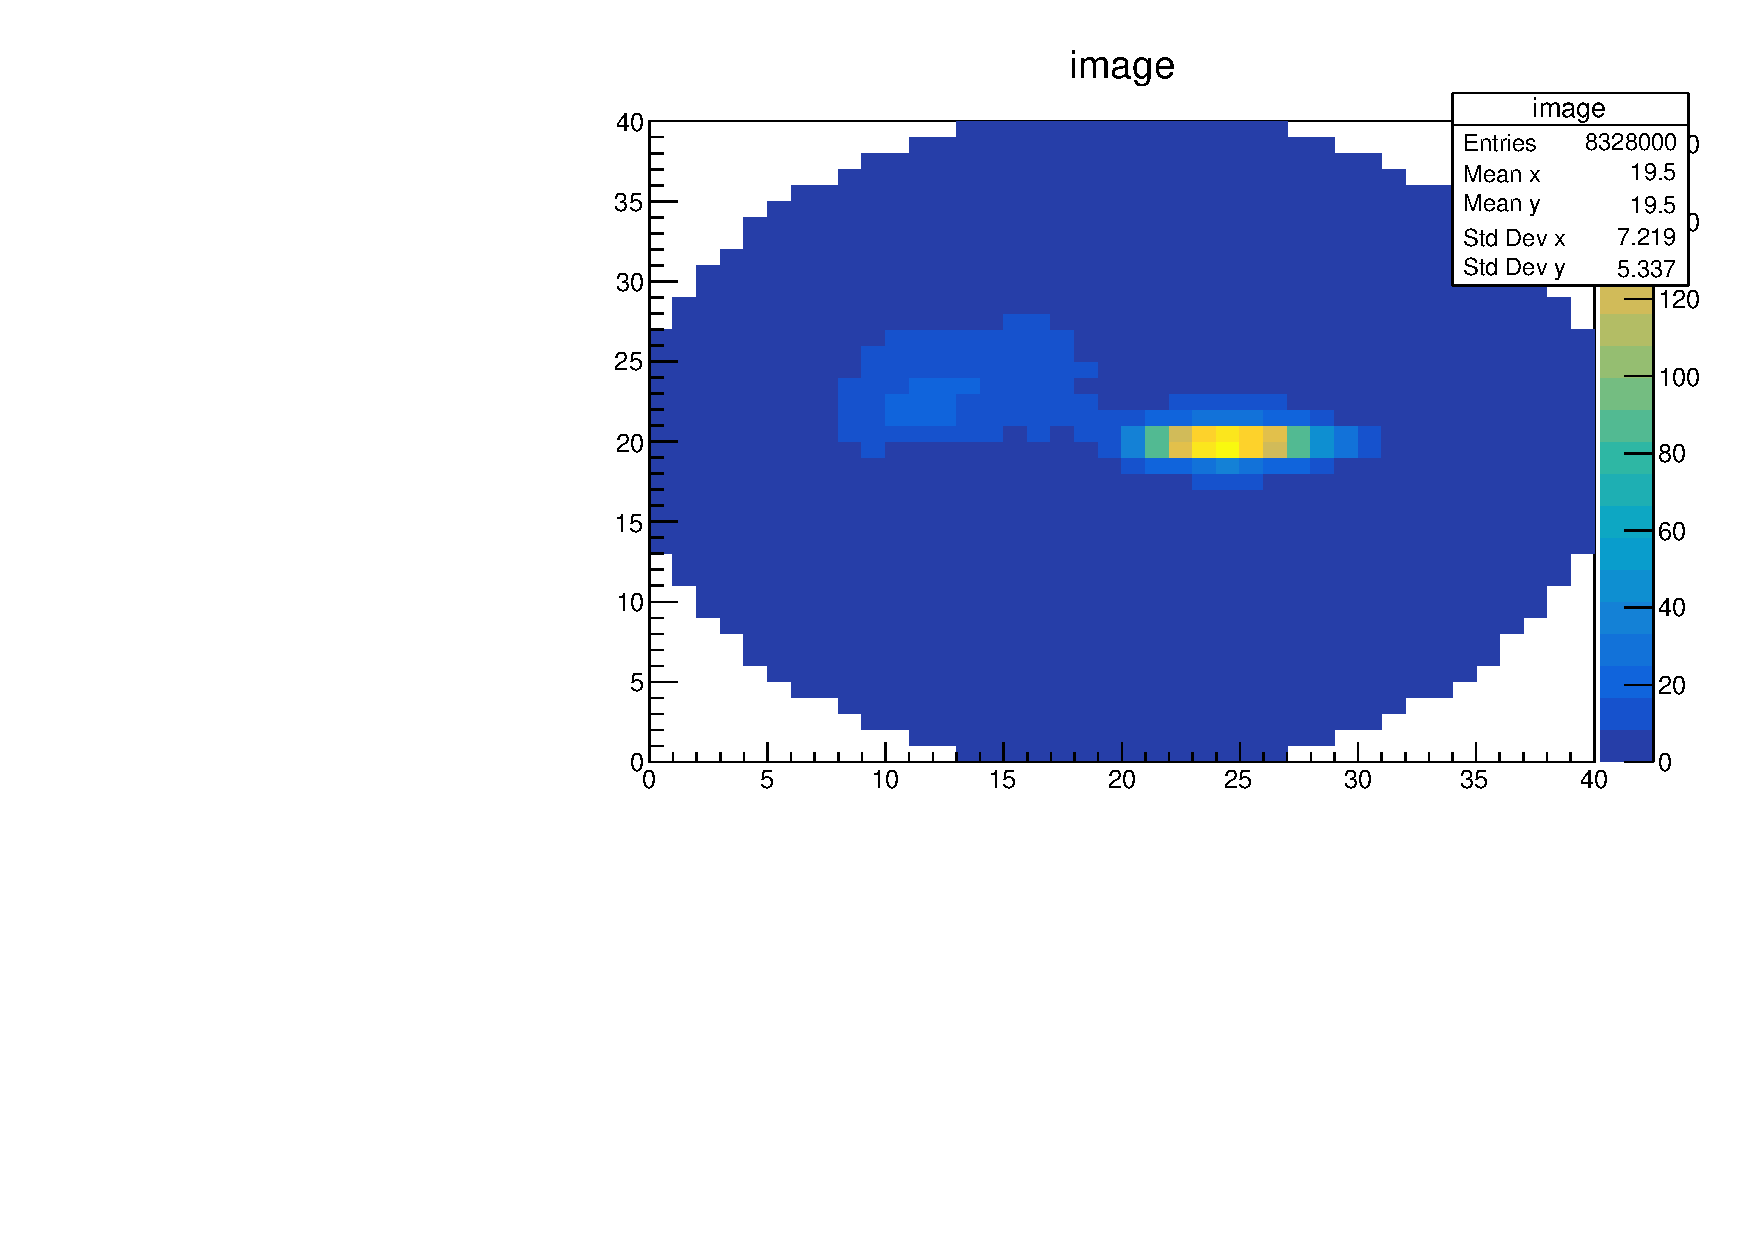
\includegraphics[width=0.32\textwidth]{./NoNorm/imageTOP.pdf}
        \end{center}
        \caption{
            Figures where $E_0 \ne 1$ GeV but the quantity $\frac{\mathbf{E_i}}{E_0}$ is used to fill the histograms.\\
            {\bf(LEFT):} QCD jets,\\
            {\bf(MIDDLE):} $W^{\pm}$ jets,\\
            {\bf(RIGHT):} Top jets.\\
            There seems to be no difference between this and \autoref{fig:case5}.
        }
        \label{fig:caseNorm}
    \end{figure}

    Image formation with a different normalization for $E_0$ is presented in \autoref{fig:caseNorm} (z axis is intentionally left unnormalized so that it can be easily compared with \autoref{fig:case5}), filling the quantity $\frac{\mathbf{E_i}}{E_0}$ correctly normalizes the image.
    
    
    
\end{document}
